\documentclass[pdf]{beamer}
\mode<presentation>{}
\usepackage{minted}
\usepackage{tikz}
\usepackage{pgffor} %% gives looping with \foreach
\usepackage[absolute,overlay]{textpos}
\usepackage{lmodern} %% scalable latin characters
\usetikzlibrary{arrows,shapes,backgrounds}
\usepackage{multirow}
\usepackage{listings} %% another package for code related stuff

%% stuff for minted
\definecolor{mintedBg}{rgb}{0.95, 0.95, 0.95}
\definecolor{blockBg}{rgb}{0.6, 0.6, 0.95}
\definecolor{rnaColor}{rgb}{0, 0.6, 0}
\definecolor{cdsColor}{rgb}{0, 0.4, 0.4}
\definecolor{rnaPol}{rgb}{0.8,0,0.8}
\definecolor{ribosomeCol}{rgb}{0.5,0.5,0.1}
\definecolor{protColor}{rgb}{0.6,0,0.6}
%% colours for nucleotides:
\definecolor{dACol}{rgb}{0.5, 0.5, 0}
\definecolor{dCCol}{rgb}{0.8, 0, 0}
\definecolor{dGCol}{rgb}{0, 0.8, 0}
\definecolor{dTCol}{rgb}{0, 0, 0.8}

\definecolor{navy}{rgb}{0, 0, 0.6}
\definecolor{pur}{rgb}{0, 0, 0.6}
\definecolor{pyr}{rgb}{0.6, 0, 0.2}

\definecolor{purple1}{rgb}{1.0, 0, 0.6}
\definecolor{purple2}{rgb}{0.8, 0, 0.8}
\definecolor{purple3}{rgb}{0.6, 0, 1.0}
%% define styles for different codes
\newminted{cpp}{linenos, bgcolor=blockBg, fontsize=\footnotesize}
%% then use \begin{cppcode}
\newminted{c}{linenos, bgcolor=mintedBg, fontsize=\footnotesize}
\newminted{perl}{linenos, bgcolor=mintedBg, fontsize=\footnotesize}

%% a command to define a subheading
\newcommand\subHeading[1]{
  \par\bigskip {\Large\bfseries#1}\par\smallskip
}

%% I detest indentation in footnotes etc, so try this:
\makeatletter
\renewcommand\@makefntext[1]{\noindent\makebox[0em][r]{\@makefnmark}\tiny#1}
\makeatother
%% the makeatletter and makeatother are required to allow me to
%% to change the macro beginning with an @. (though when I call it
%% I don't use the @ ... 

\setlength\parskip{0.5em}
\setlength\parindent{0ex}

%% to have footnotes without references. This from tex.stackexchange.com
\newcommand\blfootnote[1]{%
  \begingroup  %% this makes it a local redefinition
  \renewcommand\thefootnote{}\footnote{#1}%
  \addtocounter{footnote}{-1}  % this adjusts the footnote counter
  \endgroup
}


%% to draw a pair of genes..
\newcommand{\genePair}[3][]{
        \draw [-,#1] (#2-1,#3) -- (#2+1,#3);
        \draw [-,line width=2, purple1] (#2-0.5,#3) -- (#2+0.5,#3);
        \draw [-,#1] (#2-1,#3-0.5) -- (#2+1,#3-0.5);
        \draw [-,line width=2, purple3] (#2-0.5,#3-0.5) -- (#2+0.5,#3-0.5);  
}

\title{Finding sequence in databases}
\subtitle{aligning one sequence to many}
\author{Martin Jakt}

\begin{document}

\begin{frame}
\titlepage
\end{frame}

\begin{frame}{Identification of homologous sequences}
\begin{description}
\item[previously] identification of homologous regions within pairs or sets of
  sequences
\item[today] identification of sequences from large databases that contain
  regions of homology to a query sequence.
\end{description}
\end{frame}

\begin{frame}{When}
  \begin{itemize}
  \item Experimentally defined sequence (potentially novel
    sequence).
  \item Experimentally identified sequence (i.e. known sequence but our
    experimental results suggest some kind of interesting functionality)
  \item Specific question (e.g. a wish to identify important residues in a
    given functional motif)
  \item Classification of relationships between sequences
  \item Extension of information (we have a partial sequence and wish to
    extend it)
  \item ...
  \end{itemize}
\end{frame}

\begin{frame}{When}
In general these are similar to reasons for doing multiple sequence alignment
and the database search is often required to identify the sets of sequences to
align.

But also includes more common and simple tasks; e.g., when life presents you with a
sequence and you either don't know what it is, or you wish to extend the
sequence itself from published sequences, or to extend your understanding of
the biological role of the sequence.
\end{frame}

\begin{frame}{The questions we ask}
  \begin{itemize}
  \item Is the sequence known or novel?
  \item Can we extend it if partial (e.g. extension of expressed sequence tags
    (ESTs))?
  \item Does the sequence contain regions that are homologous to other
    sequences? (This allows us to infer some function from the sequence)
  \item Genomic coordinates of sequences (many different uses in genomics,
    e.g. mapping exons / intron locations)
  \end{itemize}
  Questions are generally asked as preludes to additional analyses, not as an
  end in themselves.

  The questions asked are changing with advances: in the old days everyone
  wanted a novel sequence; today a novel sequence probably means experimental
  error.
\end{frame}

\begin{frame}{Sequence / database types}
  Depends on purpose:
  \begin{itemize}
  \item Identify all matching sequences. Nucleotide collection (nr/nt).
    Comprehensive, including multiple sequences from same genes / transcripts.
  \item Identify all matching transcripts. Reference sequences, refseq\_rna, refseq\_protein.
  \item Identify paralogues. Genome specific databases.
  \item Identify orthologues. Several genome specific databases.\footnote{or use nr and write
      a script to filter the results}
  \item Identify genomic coordinates. Genome specific databases.
  \end{itemize}
  
  Choice of database as important as method used. 
\end{frame}

\begin{frame}{A local alignment problem}
  \begin{figure}[ht]
    \begin{tikzpicture}[scale=0.5]
      \draw [help lines, opacity=0.0] (0,0) grid (22,12);
%      \foreach \x in {1,2,...,19} \node [font=\small] at (\x,0) {\x};
%      \foreach \y in {1,2,...,12} \node [font=\small] at (20,\y) {\y};
      \visible<2->{
        \draw [-] (1,12) -- (6,12) node [midway, above, scale=0.5] {sequence A};
        \draw [-] (1.5,12.5) -- (1.5, 7) node [midway, above, rotate=90,
          scale=0.5] {sequence B};
        \draw [-, line width=1.2] (2,11.5) -- (3,10.5);
        \draw [-, line width=0.8] (4,8) -- (4.5,7.5);
      }
      \visible<3->{
        \node [right, scale=0.5, align=left, text width=12em] at (6,11)
        {sequence A and B have two homologous regions};
      }
      
      \visible<4->{
        \draw [-, rounded corners, dashed] (1.7,4.9) -- (1.7,5.1) -- (10,5.1)
        -- (10.25, 5.35) -- (10.5,5.1) -- (21,5.1) -- (21,4.9);
        \node [above, scale=0.6] at (10.25,5.25) {Database sequences};
        \draw [-] (1.5,4.3) -- (1.5, 1) node [midway, above, rotate=90,
          scale=0.5] {query};
        \draw [-] (1.7,4.5) -- (4,4.5) node [midway, above, 
          scale=0.5] {db 1};
        \draw [-] (4.2,4.5) -- (7.5,4.5) node [midway, above,
          scale=0.5] {db 2};
        \draw [-] (7.7,4.5) -- (10.3,4.5) node [midway, above,
          scale=0.5] {db 3};
        \draw [-] (10.5,4.5) -- (12.3,4.5) node [midway, above,
          scale=0.5] {db 4};
        \draw [-] (12.5,4.5) -- (15.3,4.5) node [midway, above,
          scale=0.5] {db 5};
        \draw [-] (15.5,4.5) -- (16.5,4.5) node [midway, above,
          scale=0.5] {db 6};
        \draw [-] (16.7,4.5) -- (18.5,4.5) node [midway, above,
          scale=0.5] {db 7};
        \draw [-, dotted] (18.7,4.5) -- (21,4.5);
      }
      \visible<5->{
        \draw [-, line width=1.2] (5,3.8) -- (5.4,3.4);
        \draw [-, line width=0.7] (8,3.8) -- (8.4,3.4);
        \draw [-, line width=0.4] (14.3,3.8) -- (14.7,3.4);
        \draw [-, line width=0.5] (2,2) -- (3,1);
      }
      \visible<6->{
        \node [right, scale=0.5, align=left, text width=12em] at (6,2)
        {query sequence has two distinct regions of homology};
      }
    \end{tikzpicture}
  \end{figure}
\end{frame}

\begin{frame}{What we can infer}
  \begin{figure}[ht]
    \begin{tikzpicture}[scale=0.5]
%      \draw [help lines, opacity=0] (0,0) grid (22,6);
%      \foreach \x in {1,2,...,19} \node [font=\small] at (\x,0) {\x};
%      \foreach \y in {1,2,...,6} \node [font=\small] at (20,\y) {\y};
        \draw [-, rounded corners, dashed] (1.7,4.9) -- (1.7,5.1) -- (10,5.1)
        -- (10.25, 5.35) -- (10.5,5.1) -- (21,5.1) -- (21,4.9);
        \node [above, scale=0.6] at (10.25,5.25) {Database sequences};
        \draw [-] (1.5,1) -- (1.5, 4.3) node [midway, above, rotate=90,
          scale=0.5] {query};
        \draw [-] (1.7,4.5) -- (4,4.5) node [midway, above, 
          scale=0.5] {db 1};
        \draw [-] (4.2,4.5) -- (7.5,4.5) node [midway, above,
          scale=0.5] {db 2};
        \draw [-] (7.7,4.5) -- (10.3,4.5) node [midway, above,
          scale=0.5] {db 3};
        \draw [-] (10.5,4.5) -- (12.3,4.5) node [midway, above,
          scale=0.5] {db 4};
        \draw [-] (12.5,4.5) -- (15.3,4.5) node [midway, above,
          scale=0.5] {db 5};
        \draw [-] (15.5,4.5) -- (16.5,4.5) node [midway, above,
          scale=0.5] {db 6};
        \draw [-] (16.7,4.5) -- (18.5,4.5) node [midway, above,
          scale=0.5] {db 7};
        \draw [-, dotted] (18.7,4.5) -- (21,4.5);
      
        \draw [-, line width=1.2] (5,3.8) -- (5.4,3.4);
        \draw [-, line width=0.7] (8,3.8) -- (8.4,3.4);
        \draw [-, line width=0.4] (14.3,3.8) -- (14.7,3.4);
        \draw [-, line width=0.5] (2,2) -- (3,1);
        \visible<2->{
          \draw [-, thick, red] (1.5, 3.8) -- (1.5, 3.4) node [midway, above,
            rotate=90] {a};
          \draw [-, thick, blue] (1.5, 2) -- (1.5, 1) node [midway, above,
            rotate=90] {b};
        }
    \end{tikzpicture}
  \end{figure}
  \visible<2->{
    {\small
      \begin{itemize}
      \item The query sequence contains two regions \textcolor{red}{a} and
        \textcolor{blue}{b} which are homologous to distinct sequences.
      \item Region \textcolor{red}{a} can be found in multiple sequences and is
        likely to represent a functional domain.
      \item Region \textcolor{blue}{b} was only found in a single other sequence,
        and may represent a common origin (i.e. an evolutionary relationship) that
        does not necessarily imply function.
      \end{itemize}
    }
  }
\end{frame}

\begin{frame}{How can we do this}
  In theory, dynamic programming (e.g. Smith-Waterman) could be used against
  the database. However, the databases are usually too big for this to be
  reasonable.\footnote{Depends on the database though and the FASTA
    suite includes full Smith-Waterman based search programs.}

  Instead \textcolor{blue}{\emph{indexed heuristic}} methods have been
  developed that allow rapid identification of homologous sequences.

  These do not guarantee the identification of all homologous sequences, but
  are fast enough to be useful, and in practice find the vast majority of
  homologous sequences.
\end{frame}

\begin{frame}{What is an index?}
  A (sorted) lookup table.\\

  eg:

  {%\fontsize{12}{1}
   % \selectfont
    \tiny
    \setlength{\tabcolsep}{0.5em}    
    \begin{tabular}{ l*{15}{|l} }
      letter & A &  & l & o & o & k & u & p & & t & a & b & l & e & . \\
      \hline
      position & 1 & 2 & 3 & 4 & 5 & 6 & 7 & 8 & 9 & 10 & 11 & 12 & 13 & 14 & 15 \\
    \end{tabular}
    \visible<2->{
      \begin{tabular}{ l|l }
        letter & position \\
        . & 15 \\
        & 2,9 \\
        A & 1 \\
        a & 11 \\
        b & 12 \\
        e & 14 \\
        k & 6 \\
        l & 3,13 \\
        o & 4,5 \\
        p & 8 \\
        t & 10 \\
        u & 7 \\
      \end{tabular}
    }
  }

  \visible<3>{
    many different kinds of indices possible.
  }
\end{frame}

\begin{frame}{What is a heuristic?}
  \begin{itemize}
  \item A method that does not guarantee an optimal solution
  \item Generally faster than optimal methods
  \item Does not require proof of optimality (i.e. does not require deep
    maths)
  \item Does something that seems reasonable
  \item Assessed empirically (i.e. run the methods on different data sets and
    try to measure how well it works).
  \end{itemize}
\end{frame}

\begin{frame}{Database searching methods}
  \begin{description}
    \item[FASTA] The first generally useful method. Uses k-tuple word lookup
      tables.
    \item[BLAST] The second method. Indexes the query sequence and compares
      the database to this index. The most widely used method by far due to
      the combination of sensitivity and speed.
    \item[BLAT] The third method. Extremely fast performance ($\sim$1000s x
      faster than BLAST) due to indexing the database. Lower sensitivity to divergent
      sequences. Primarily used to find exact or near exact matches to
      nucleotide sequences.
    \item[BWT] A series of methods using indexes based on the Burrows-Wheeler
      transform. Extremely fast, but like BLAT used primarily for mapping
      exact sequences to databases. Used primarily to map next generation
      sequencing (NGS) to genome locations.
  \end{description}
\end{frame}

\begin{frame}{FASTA}
  Originally designed for protein sequences (FASTP), then generalised to
  include any kind of sequences. P for protein, A, for All.

  Original method see:\\
  Rapid and Sensitive Protein Similarity Searches\\
  Lipman and Pearson, Science 1985, 227; 4693. pp 1435-1441\\
  \emph{Eminently readable paper}

  Extension:\\
  Improved tools for biological sequence comparison\\
  Pearson and Lipman, PNAS 1988, 85; 8. pp 2444-2448 
\end{frame}

\begin{frame}[fragile]{FASTA continued}
  \begin{columns}
    \begin{column}[t]{0.5\textwidth}
      {\tiny
        \setlength{\tabcolsep}{0.5em}
      \begin{tabular}{c*{7}{l}}
        Sequence & \multicolumn{7}{c}{Position}\\
        number & 1 & 2 & 3 & 4 & 5 & 6 & 7\\
        1 & F & L & W & R & T & W & S\\
        2 & S & W & K & T & W & T & \\
      \end{tabular}
      }
      \vspace{2ex}

      \pause
      A lookup table is made for sequence 1:
      
      \vspace{2ex}
      {\tiny
        \setlength{\tabcolsep}{0.5em}
      \begin{tabular}{l|l}
        AA & pos \\
        \hline
        F & 1 \\
        L & 2 \\
        W & 3,6 \\
        R & 4 \\
        T & 5 \\
        S & 7 \\
      \end{tabular}
      }
      \pause

      \vspace{2ex}
      Go through each position in sequence 2 and calculate offsets for the AAs.
      \end{column}
    \begin{column}[t]{0.5\textwidth}
      {\tiny
        \setlength{\tabcolsep}{0.5em}
        \begin{tabular}{l|ll|l}
          AA & S2 & S1 & S1-S2 \\
          \hline
          S & 1 & 7 & 6\\
          W & 2 & 3,6 & 1,4\\
          K & 3 & & \\
          T & 4 & 5 & 1\\
          W & 5 & 3,6 & -2,1\\
          T & 6 & 5 & -1\\
        \end{tabular}
      }
      \pause

      \vspace{2ex}
      {\small
      Most common offset: 1, suggests an alignment of sequence 2 offset by 1
      starting at position two:

\begin{verbatim}
  S1: WRTW
      | ||
  S2: WKTW      
\end{verbatim}
      
      Took N steps to find potential non-gapped alignment where N is the
      length of sequence 2.
    }
    \end{column}
  \end{columns}
  {\small
  \emph{For protein sequences, k usually 1 or 2.}
  }
\end{frame}

\begin{frame}{Fasta continued}
  Seed and extend:
  \begin{columns}
    \begin{column}{0.5\textwidth}
      \includegraphics[width=\textwidth]{images/Fasta_four_steps_b}

      {\tiny (From 1988 PNAS paper)}
    \end{column}
    \begin{column}{0.6\textwidth}
      {\footnotesize
      \begin{description}
      \item[A] Identify regions of similarity (k-tup lookup table).
      \item[B] Scan regions using scoring matrix; save the best regions.
      \item[C] Join initial regions if it improves alignments scores.
      \item[D] Recalculate optimised alignment centered around the highest
        scoring region (modified Needleman-Wunsh / Smith-Waterman).
      \end{description}
      }
    \end{column}
  \end{columns}
  {\tiny Many steps, but much faster than optimal method.}
\end{frame}

\begin{frame}{When should you use FASTA}

  {\small
  The FASTA algorithm has to a large extent been overtaken by BLAST and it's
  many incarnations (due to speed). However, the FASTA programs are more
  flexible and may offer superior sensitivity:
  }
  {\tiny
    \begin{enumerate}
    \item Rigorous algorithms unavailable in BLAST (Table I). Smith-Waterman
      (ssearch36), global: global (ggsearch36), and global:local (glsearch36)
      programs are available, and these programs can be used with psiblast PSSM profiles.
    \item Better translated alignments. fastx36, fasty36, tfastx36, and tfastx36
      allow frame-shifts in alignments; frame-shifts are treated like gap-penalties,
      alignments tend to be longer in error-prone reads.
    \item Better statistics. BLAST calculates very accurate statistics for
      protein:protein alignments, but its model-based strategy is less robust
      for translated-DNA:protein and DNA:DNA scores. FASTA uses an empirical
      estimation strategy, and now provides both search-based, and
      high-scoring shuffle-based statistics (-z 21).
    \item More flexible library sequence formats. The FASTA programs can read FASTA,
      NCBI/formatdb, and several other sequence formats, and can directly query MySQL and
      Postgres databases. The programs offer several strategies for specifying subsets
      of databases.
    \item A very efficient threaded implementation. The FASTA programs are fully
      threaded; both similarity scores and alignments can be calculated in parallel on multi-core
      hardware. On multi-core machines, FASTA can be faster than BLAST while producing better
      alignments with more accurate statistical estimates.
    \item A powerful annotation facility. The FASTA programs can incorporate
      functional site annotations, site variation, and domain-based sub-alignment scoring using
      annotations from sequence libraries. Scripts are available to download site and domain
      information from Uniprot, and domain information fromk Pfam and
      CATH. Domain information can be used to sub-divide alignment scores to
      ensure that the aligned domain is homologous.
    \end{enumerate}
    (Taken directly from fasta\_guide for fasta-36.3.8)
  }

  \small Suitable if you understand the requirements of your problem.
\end{frame}

\begin{frame}{BLAST}
  \textcolor{blue}{B}asic \textcolor{blue}{L}ocal \textcolor{blue}{A}lignment
  \textcolor{blue}{S}earch \textcolor{blue}{T}ool:

  The standard sequence search tool.

  Altschul, Gish, Miller, Myers, Lipman. Journal of Molecular Biology 1990,
  5;215(3), pp. 403-410.

  \emph{not as easy a read as the FASTP paper, but not too bad}
\end{frame}

\begin{frame}{the BLAST algorithm}

  {\small
  Search non-overlapping words of a database of sequences against an index of
  high-scoring (as determined by an amino-acid substitution matrix) words
  present in the query sequence.

  \begin{enumerate}
  \item Create an index of high scoring (overlapping) words ($w$-mers) in a sequence:
    \begin{itemize}
      \item \textcolor{blue}{protein}: $w$-mers of the sequence and mutations of these whose
        alignment scores exceed a given threshold T. $\sim$50 words per
        residue (for $w$ of 4).
      \item \textcolor{blue}{DNA}: all overlapping $w$-mers ($w$, typically being 11). Hence,
        n-$w$+1 words for a sequence of length n.
    \end{itemize}
  \item Scan all non-overlapping words of the database sequences against this
    index.
  \item Extend hits residue by residue until the score falls below a threshold
    based upon the maximum score obtained in the extension.
  \end{enumerate}
  
  Scores are simply the sums of match / mismatch scores from an amino acid
  substitution matrix or for DNA fixed match / mismatch. 
  }
\end{frame}

\begin{frame}[fragile]{the BLAST algorithm...}
  \begin{figure}[ht]
    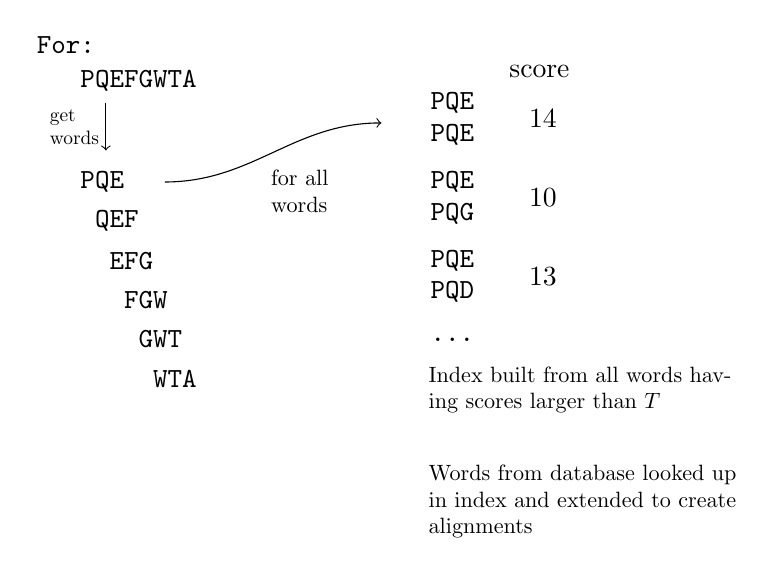
\begin{tikzpicture}[scale=0.5]
%      \draw [help lines, opacity=0.5] (0,0) grid (22,12);
%      \foreach \x in {1,2,...,19} \node [font=\small] at (\x,0) {\x};
%      \foreach \y in {1,2,...,12} \node [font=\small] at (20,\y) {\y};
      \node [font=\ttfamily, right, align=left] at (1,12) {For:\\ \verb|   PQEFGWTA|};
%      \visible<2->{
        \draw [->] (3,11) -- (3,9.8) node [midway, left, scale=0.7, align=left] {get\\words};
        \node [right] at (1,9) {\verb|   PQE|};
        \node [right] at (1,8) {\verb|    QEF|};
        \node [right] at (1,7) {\verb|     EFG|};
        \node [right] at (1,6) {\verb|      FGW|};
        \node [right] at (1,5) {\verb|       GWT|};
        \node [right] at (1,4) {\verb|        WTA|};
%      }
%      \visible<3->{
%        \draw [->] (4.5,9) to [out=0,in=180] (7,9) to [out=0,in=180] (10,10.5);
        \draw [->] (4.5,9) to [out=0,in=180] (10,10.5);
        \node [below right, align=left, scale=0.8] at (7,9.5) {for all\\words};
        \node [right] at (11,11) {\verb|PQE|};
        \node [right] at (11,10.2) {\verb|PQE|};
        \node [right] at (13.5,10.6) {14};

        \node [right] at (11,9) {\verb|PQE|};
        \node [right] at (11,8.2) {\verb|PQG|};
        \node [right] at (13.5,8.6) {10};

        \node [right] at (11,7) {\verb|PQE|};
        \node [right] at (11,6.2) {\verb|PQD|};
        \node [right] at (13.5,6.6) {13};
        
        \node [right] at (13,11.8) {score};
        \node [right] at (11,5) {\verb|...|};

        \node [below right, scale=0.8, align=left, text width=5cm] at (11,4.5)
        {Index built from all words having scores larger than $T$};

        \node [below right, scale=0.8, align=left, text width=5cm] at (11,2)
        {Words from database looked up in index and extended to create
        alignments};

%      }
    \end{tikzpicture}
  \end{figure}
\end{frame}

\begin{frame}{BLAST variants}
  \begin{description}
  \item[blastn] nucleotide query vs nucleotide database
  \item[blastp] protein sequence vs protein database
  \item[blastx] translated nucleotide query vs protein database
  \item[tblastn] protein query sequence against translated nucleotide database
  \item[tblastx] translated nucleotide query vs translated nucleotide database
  \end{description}
  
  Translated queries are done in 6 frames, and hence expensive.

  Early versions provided non-gapped alignments only.

  Many specialised variants, see:\\
  \url{http://blast.ncbi.nlm.nih.gov/Blast.cgi}\\
  Most important perhaps: PSI-blast (position specific iterated blast).
\end{frame}

\begin{frame}{An example search}

  {\tiny
  \url{http://blast.ncbi.nlm.nih.gov/Blast.cgi?PROGRAM=blastn&PAGE\_TYPE=BlastSearch&LINK\_LOC=blasthome}
  }
  \includegraphics[width=\textwidth]{images/blast_input.png}
\end{frame}

\begin{frame}{A result summary}
  \includegraphics[width=0.7\textwidth]{images/blast_graphical_overview.png}
\end{frame}

\begin{frame}{The alignment list}
  \includegraphics[width=\textwidth]{images/blast_result_list}
\end{frame}

\begin{frame}{What to look for}
  \begin{itemize}
  \item E-value: the number of random hits in this database expected at this
    score from the searched database.
  \item Query coverage: how much of the query (input) sequence is covered by
    the identified alignment.
  \item Ident: percentage identity.
  \item Alignment score.
  \end{itemize}

  What values are significant depends on the question asked.
\end{frame}

\begin{frame}{Which database}
  Olden days: NR (non-redundant) was the choice as this is the most
  complete sequence database. 

  These days: Many options depending on the choice. NR often gives too many
  matches which represent the same sequence (i.e. derived from the same gene
  in the same organism) to be reasonable. (See previous slide).

  For most queries the use of genome specific or genome assembly
  (e.g. Ensembl) databases is more appropriate.

  Unless you have generated your own sequence, the blast search is likely to
  have been already performed by the genome database, or the protein domain people.
\end{frame}

\begin{frame}{Nucleotide databases}
  at NCBI (\url{http://blast.ncbi.nlm.nih.gov/})
  \begin{itemize}
    \item Human genomic plus transcripts
    \item Mouse genomic plus transcripts
    \item Nucleotide collection (nr/nt) (big and horrible)
    \item Reference RNA sequences (refseq\_rna) (useful)
    \item Reference genomic sequences (refseq\_genomic)
    \item NCBI Genomes (chromosomes)
    \item Expressed sequence tags (est)
    \item Genomic survey sequences (gss)
    \item High throughput genomic sequences (HTGS)
    \item ...
  \end{itemize}
\end{frame}

\begin{frame}{BLAT}
  \textcolor{blue}{B}last \textcolor{blue}{L}ike \textcolor{blue}{A}lignment
  \textcolor{blue}{T}ool.
  
  James Kent, Genome Research 2002, 12:654-664.\\
  \emph{very readable paper}

  Designed to aid in the annotation of the human genome; to map ESTs and mouse
  genome sequences against the human genome.
\end{frame}

\begin{frame}{The BLAT algorithm}
  \begin{itemize}
    \item Similar to BLAST; rapidly scans for short matches and extends these
      into high scoring pairs.
    \item Builds an index of the database and then scans the query
      sequences.\footnote{
        This was tried for the initial BLAST algorithm, but was not efficient
        with the computational power available then. Note that this is also
        more problematic for the nr/nt database than for complete genome sequences}
    \item Extends any perfect or near-perfect hits
    \item Stitches together adjacent alignments into larger alignments
      effectively 'unsplicing' transcripts onto genome sequences
      (esp. useful for mapping transcript sequences to genomes).
    \item Large index, requires a memory approximately the size of the genome
      ($\sim$1 byte / base).
  \end{itemize}
\end{frame}

\begin{frame}{When to use BLAT}
  \begin{itemize}
  \item Mapping near identical sequences to each other.
  \item BLAT is fantastic for mapping spliced transcripts to genomes.
  \item As a preliminary step to map all easily mapped sequences, 
    followed by more exhaustive algorithms.
  \end{itemize}
  
  In general if you've only got a few sequences use BLAST, unless you're
  mapping transcripts to genomes.
\end{frame}

\end{document}
